%%%%%%
%
% $Autor: Wings $
% $Datum: 2020-01-18 11:15:45Z $
% $Pfad: WuSt/Skript/Produktspezifikation/powerpoint/ImageProcessing.tex $
% $Version: 4620 $
%
%%%%%%


\section{Grenzen der Künstlichen Intelligenz}

Die Bilderkennung hat in den letzten Jahren riesige Fortschritte gemacht \cite{}. Trotzdem zeigen sich auch Grenzen. In diesem Zusammenhang wird das Bild eines Pandas aus einem Paper von Ian Goodfellow und anderen Forschern gezeigt \cite{Goodfellow:2014}. Ein Algorithmus identifiziert den Panda mit einer Wahrscheinlichkeit von 57{,}7\%. Wird das Bild mit einem zweiten Bild, das der Mensch als Rauschen wahrnimmt, überlagert, so wird ein Gibbon mit einer Wahrscheinlichkeit von 99{,}3 erkannt, obwohl in den Augen eines Menschen sich das Bild nicht geändert hat. Die Situation ist in Abbildung~\ref{Adversarial:Panda} dargestellt.

\begin{figure}
    \includegraphics[page=3,width=0.9\textwidth,viewport=20 600 560 900,clip]{../../MLbib/Adversarial/1412.6572.pdf}
    
    \caption{Überlagerung des Bilds eines Pandas mit Rauschen  \cite{Goodfellow:2014}}\label{Adversarial:Panda}
\end{figure}

Das Beispiel mit dem Panda ist harmlos. Dagegen können die Auswirkungen im Straßenverkehr verheerend sein. Untersuchungen zeigen, dass durch einfache Manipulation von Verkehrsschildern Künstliche Intelligenz falsche Interpretationen durchführen. \cite{Sitawarin:2018} Durch gezielte Veränderungen eines Bilds können wohldefinierte Manipulationen durchgeführt werden. In der Abbildung~\ref{Adversarial:Stop} wird ein Schild, das ein Tempolimit markiert, durch zusätzliche Flecken in ein Stoppschild verwandelt. 



\begin{figure}
  \centering
  \includegraphics[page=2,width=0.4\textwidth,viewport=20 450 180 600,clip]{../../MLbib/Adversarial/1802.06430.pdf}
    
  \caption{Manipulation von Verkehrsschildern  \cite{Sitawarin:2018}}\label{Adversarial:Stop}
\end{figure}

Umgekehrt kann man aus den neuronalen Netzen ein optimales Bild ermittelt, dass ein Ergebnis mit einer Wahrscheinlichkeit nahe bei 100\% liefert. Dabei entstehen auch Bilder, die das menschliche Auge nicht also solches erkennen könnte. Ein klassisches Beispiel ist der Toaster in der Abbildung~\ref{Adversarial:Toaster}.\cite{Brown:2017}


\begin{figure}
    \includegraphics[page=2,width=0.9\textwidth,viewport=20 470 560 900,clip]{../../MLbib/Adversarial/1712.09665.pdf}
    
    \caption{Optimales Bild zur Identifikation eines Toasters  \cite{Sitawarin:2018}}\label{Adversarial:Toaster}
\end{figure}

